\section{Introduction}

\begin{frame}{Representations of urban spaces}
	\centering
	\scriptsize
	
	\begin{minipage}{0.5\linewidth}
		\centering
		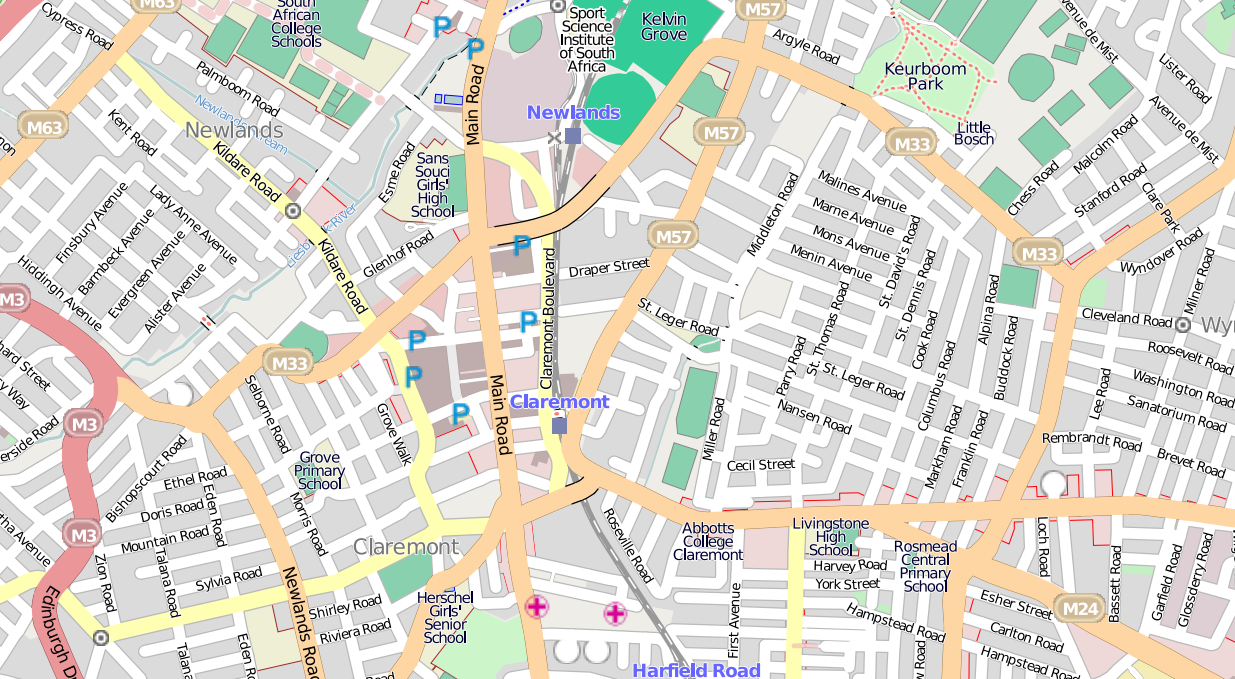
\includegraphics[width=0.9\linewidth]{context/maps}\\
		2D maps
	\end{minipage}%	
	\begin{minipage}{0.5\linewidth}
		\centering
		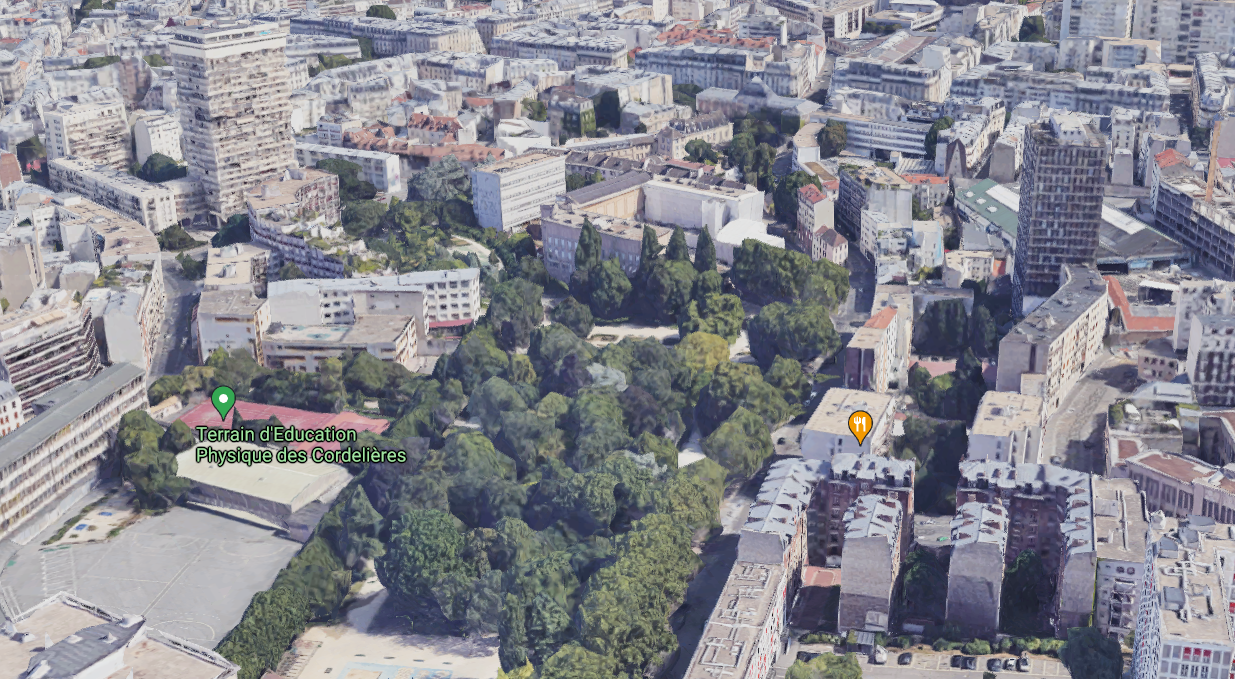
\includegraphics[width=0.9\linewidth]{context/dense_visu}\\
		3D visualization
	\end{minipage}
	
	\begin{minipage}{0.5\linewidth}
		\centering
		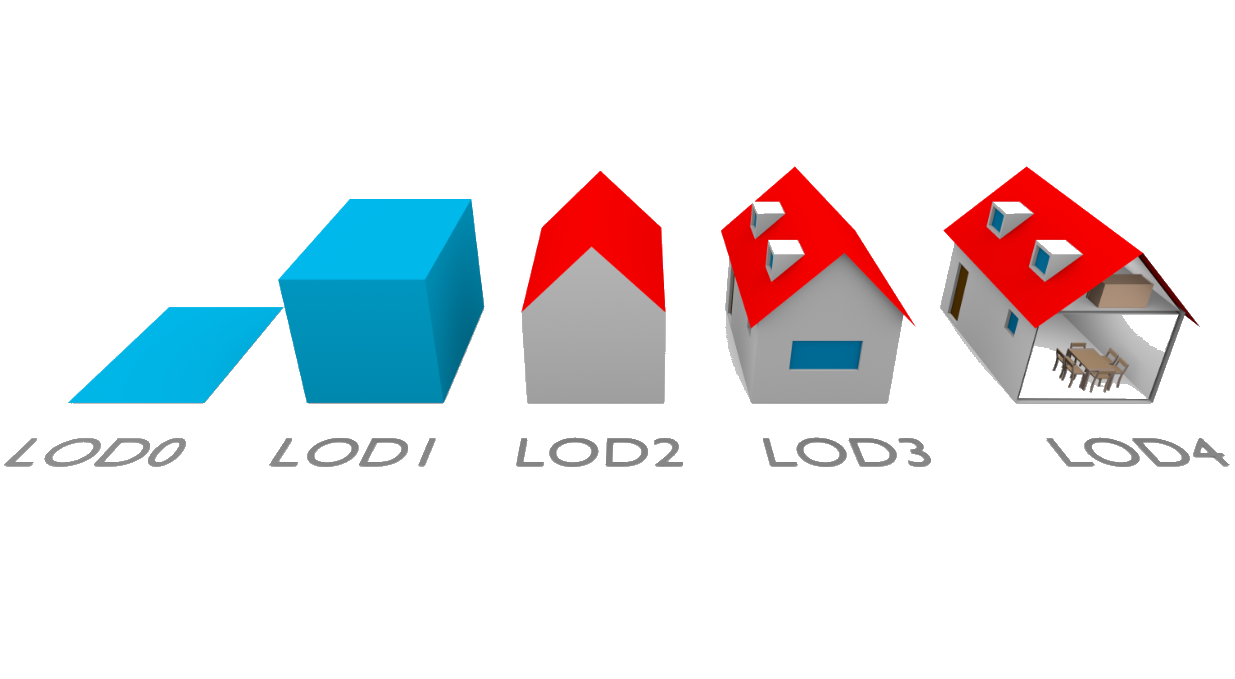
\includegraphics[width=0.9\linewidth]{context/lods}\\
		Geographic Information Systems (GIS)
	\end{minipage}%
	\begin{minipage}{0.5\linewidth}
		\centering
		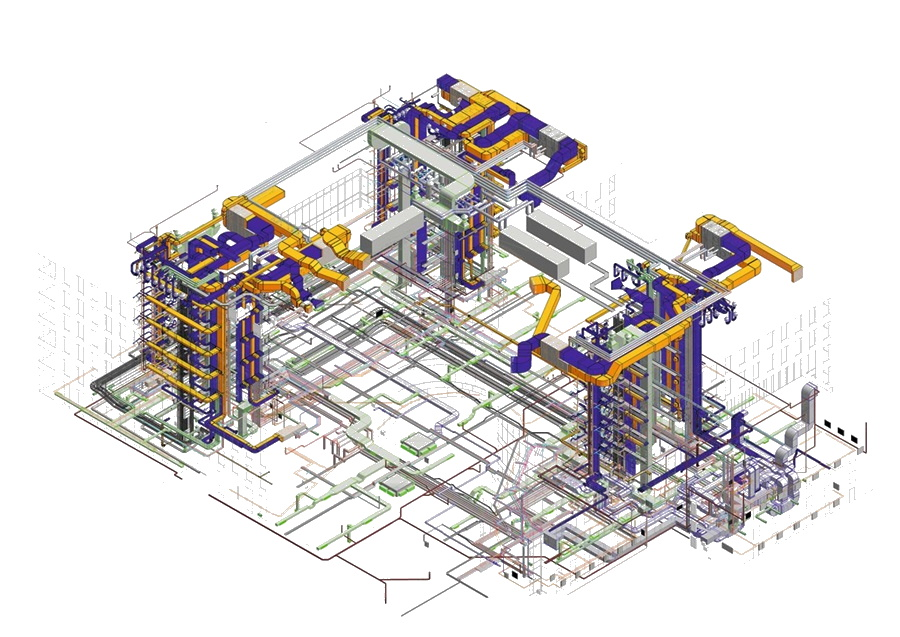
\includegraphics[width=0.9\linewidth]{context/bim}\\
		Building information model (BIM)
	\end{minipage}
\end{frame}

\begin{frame}[t]{The need for 3D models}
	\scriptsize
	\textbf{Simulation}
	\begin{figure}
		\centering
		\begin{subfigure}[t]{0.3\linewidth}
			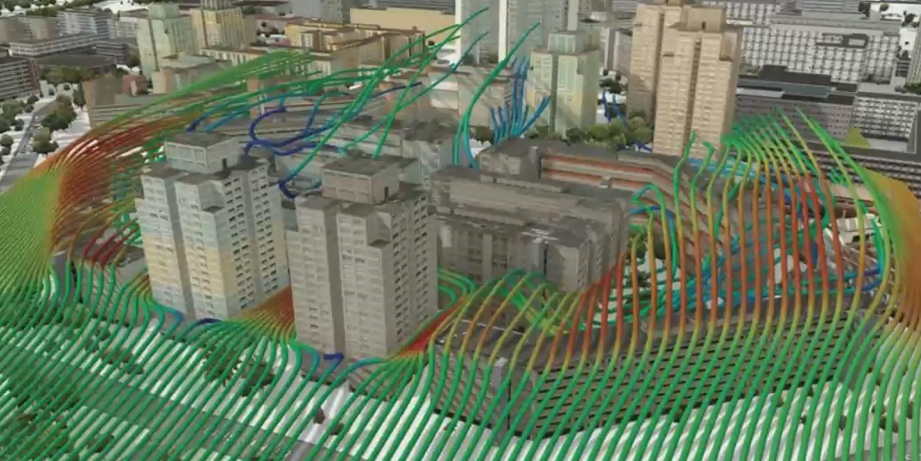
\includegraphics[width=\linewidth]{context/simulation_wind}
			\subcaption*{Wind simulation \footnote[frame]{SIMULIA, Dassault Systèmes}}
		\end{subfigure}
		\hspace{0.1\linewidth}
		\begin{subfigure}[t]{0.3\linewidth}
			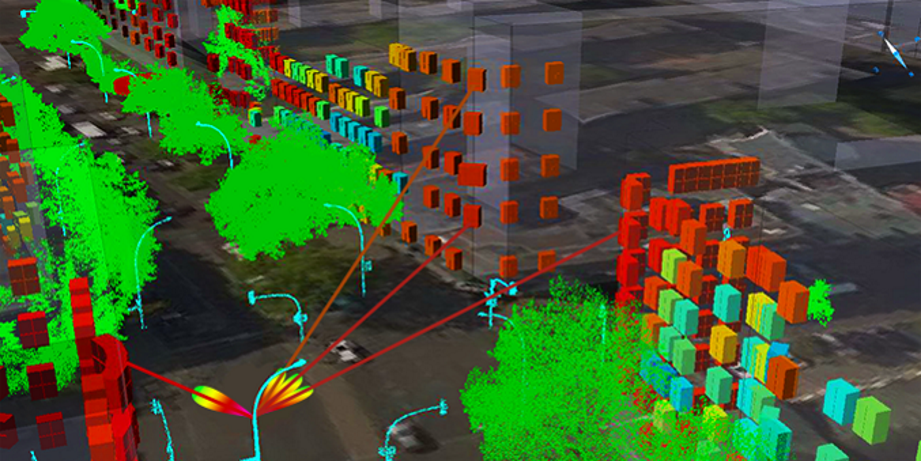
\includegraphics[width=\linewidth]{context/simulation_lineofsight}
			\subcaption*{5G connectivity \footnote[frame]{SIRADEL}}
		\end{subfigure}
	\end{figure}

	\textbf{Change tracking}
	\begin{figure}
		\centering
		\begin{subfigure}[t]{0.3\linewidth}
			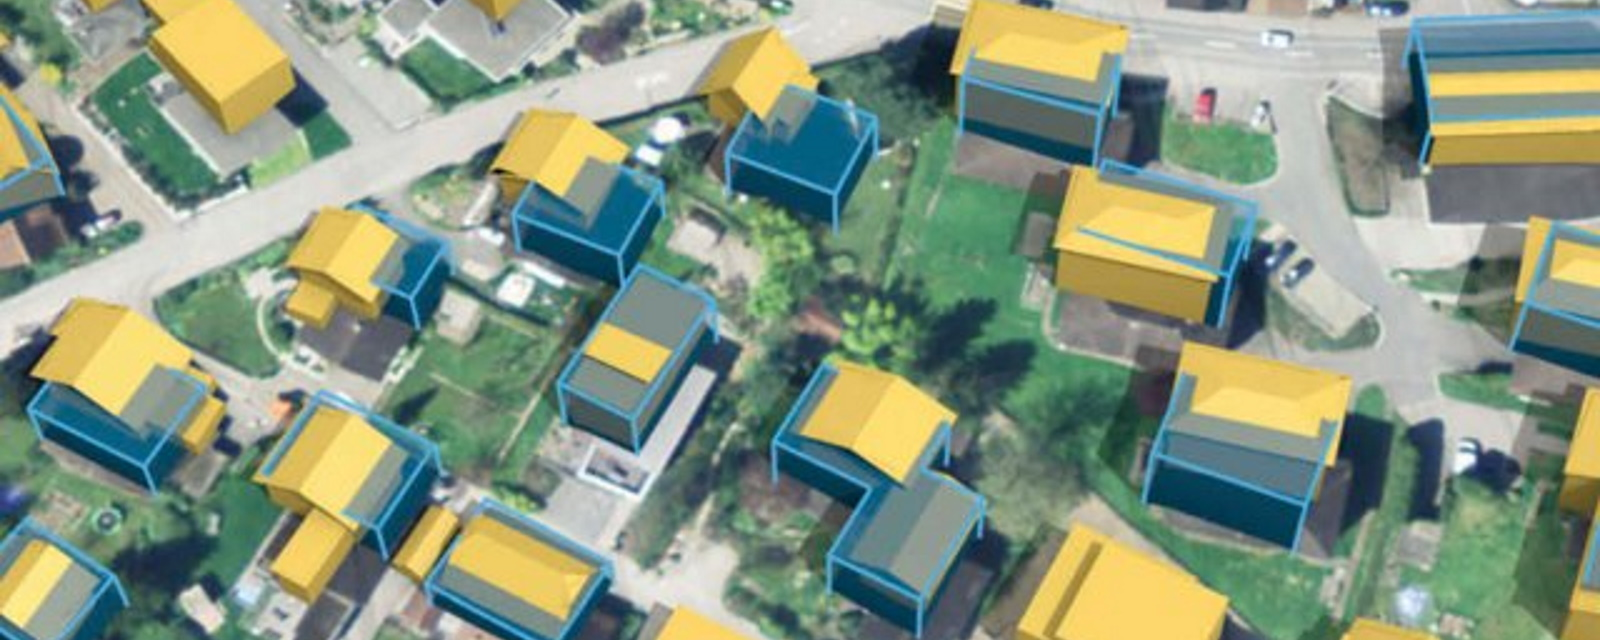
\includegraphics[width=\linewidth]{context/lod_diff_v2}
			\subcaption*{Permit verification \footnote[frame]{Taken from \cite{biljecki_EffectAcquisition_2018}}}
		\end{subfigure}
		\hspace{0.1\linewidth}
		\begin{subfigure}[t]{0.3\linewidth}
			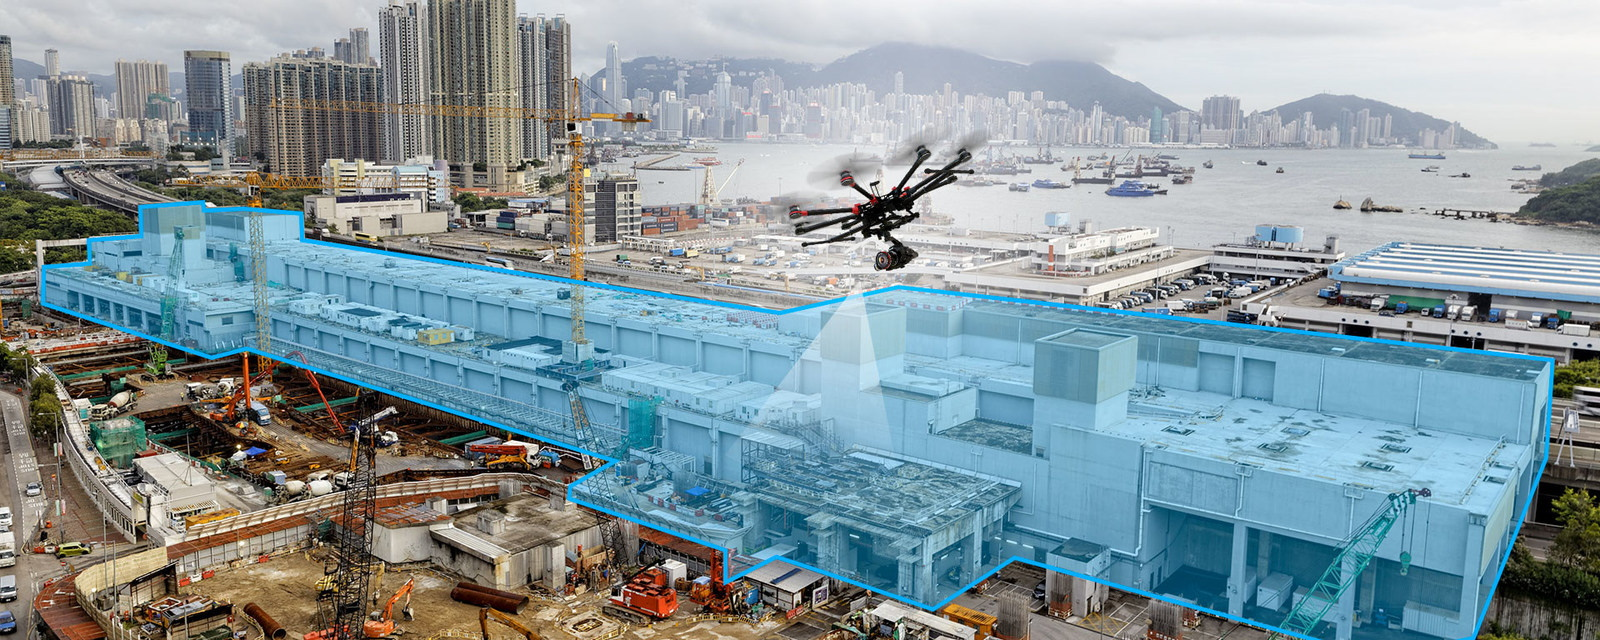
\includegraphics[width=\linewidth]{context/building_inspection}
			\subcaption*{Building inspection \footnote[frame]{\href{https://www.engineering.com/story/automating-facility-inspection-with-drones}{Engineering.com \ExternalLink}}}
		\end{subfigure}
	\end{figure}
\end{frame}

\begin{frame}{Acquisitions}
	\small
	\centering
	\begin{minipage}{0.5\linewidth}
		\centering
		\textbf{LiDAR technologies}
	\end{minipage}%
	\begin{minipage}{0.5\linewidth}
		\centering
		\textbf{Photogrammetry}
	\end{minipage}

	\begin{minipage}{0.5\linewidth}
		\centering
		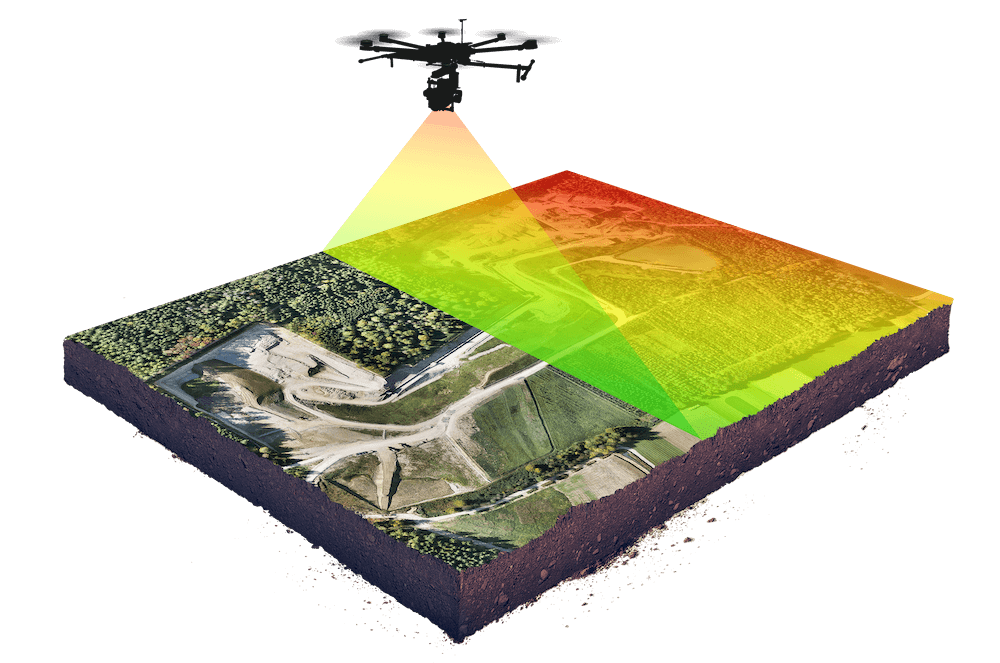
\includegraphics[width=0.7\linewidth]{context/lidar_method}			
	\end{minipage}%
	\begin{minipage}{0.5\linewidth}
		\centering
		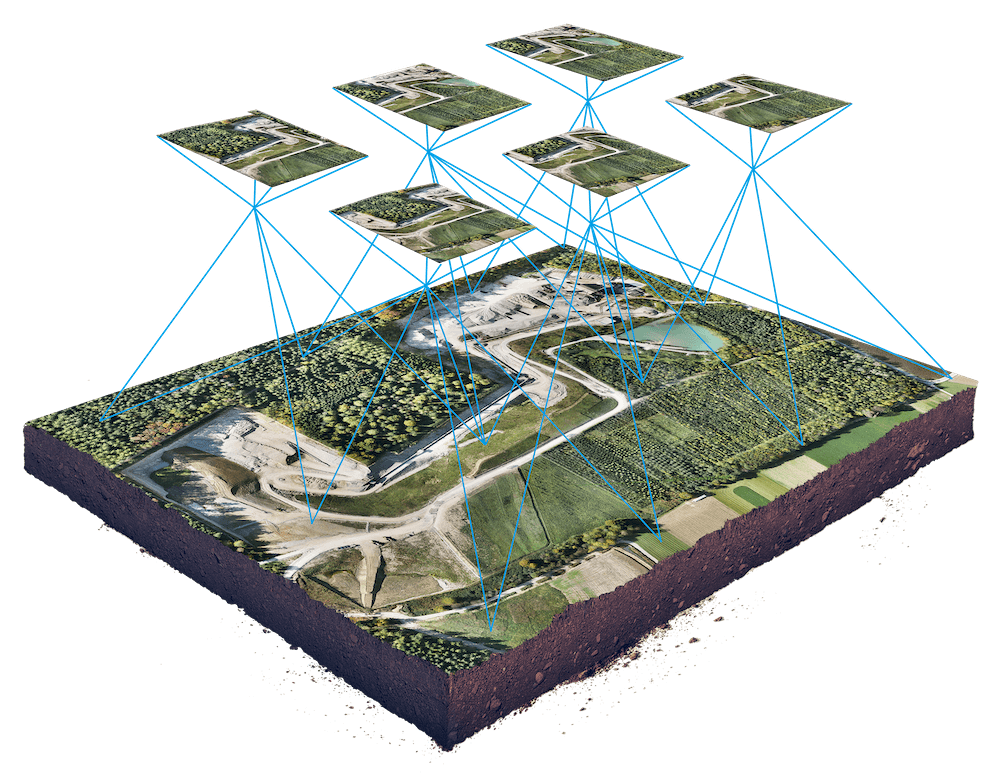
\includegraphics[width=0.7\linewidth]{context/photo_method}
	\end{minipage}

	\begin{minipage}{0.5\linewidth}
		\centering
		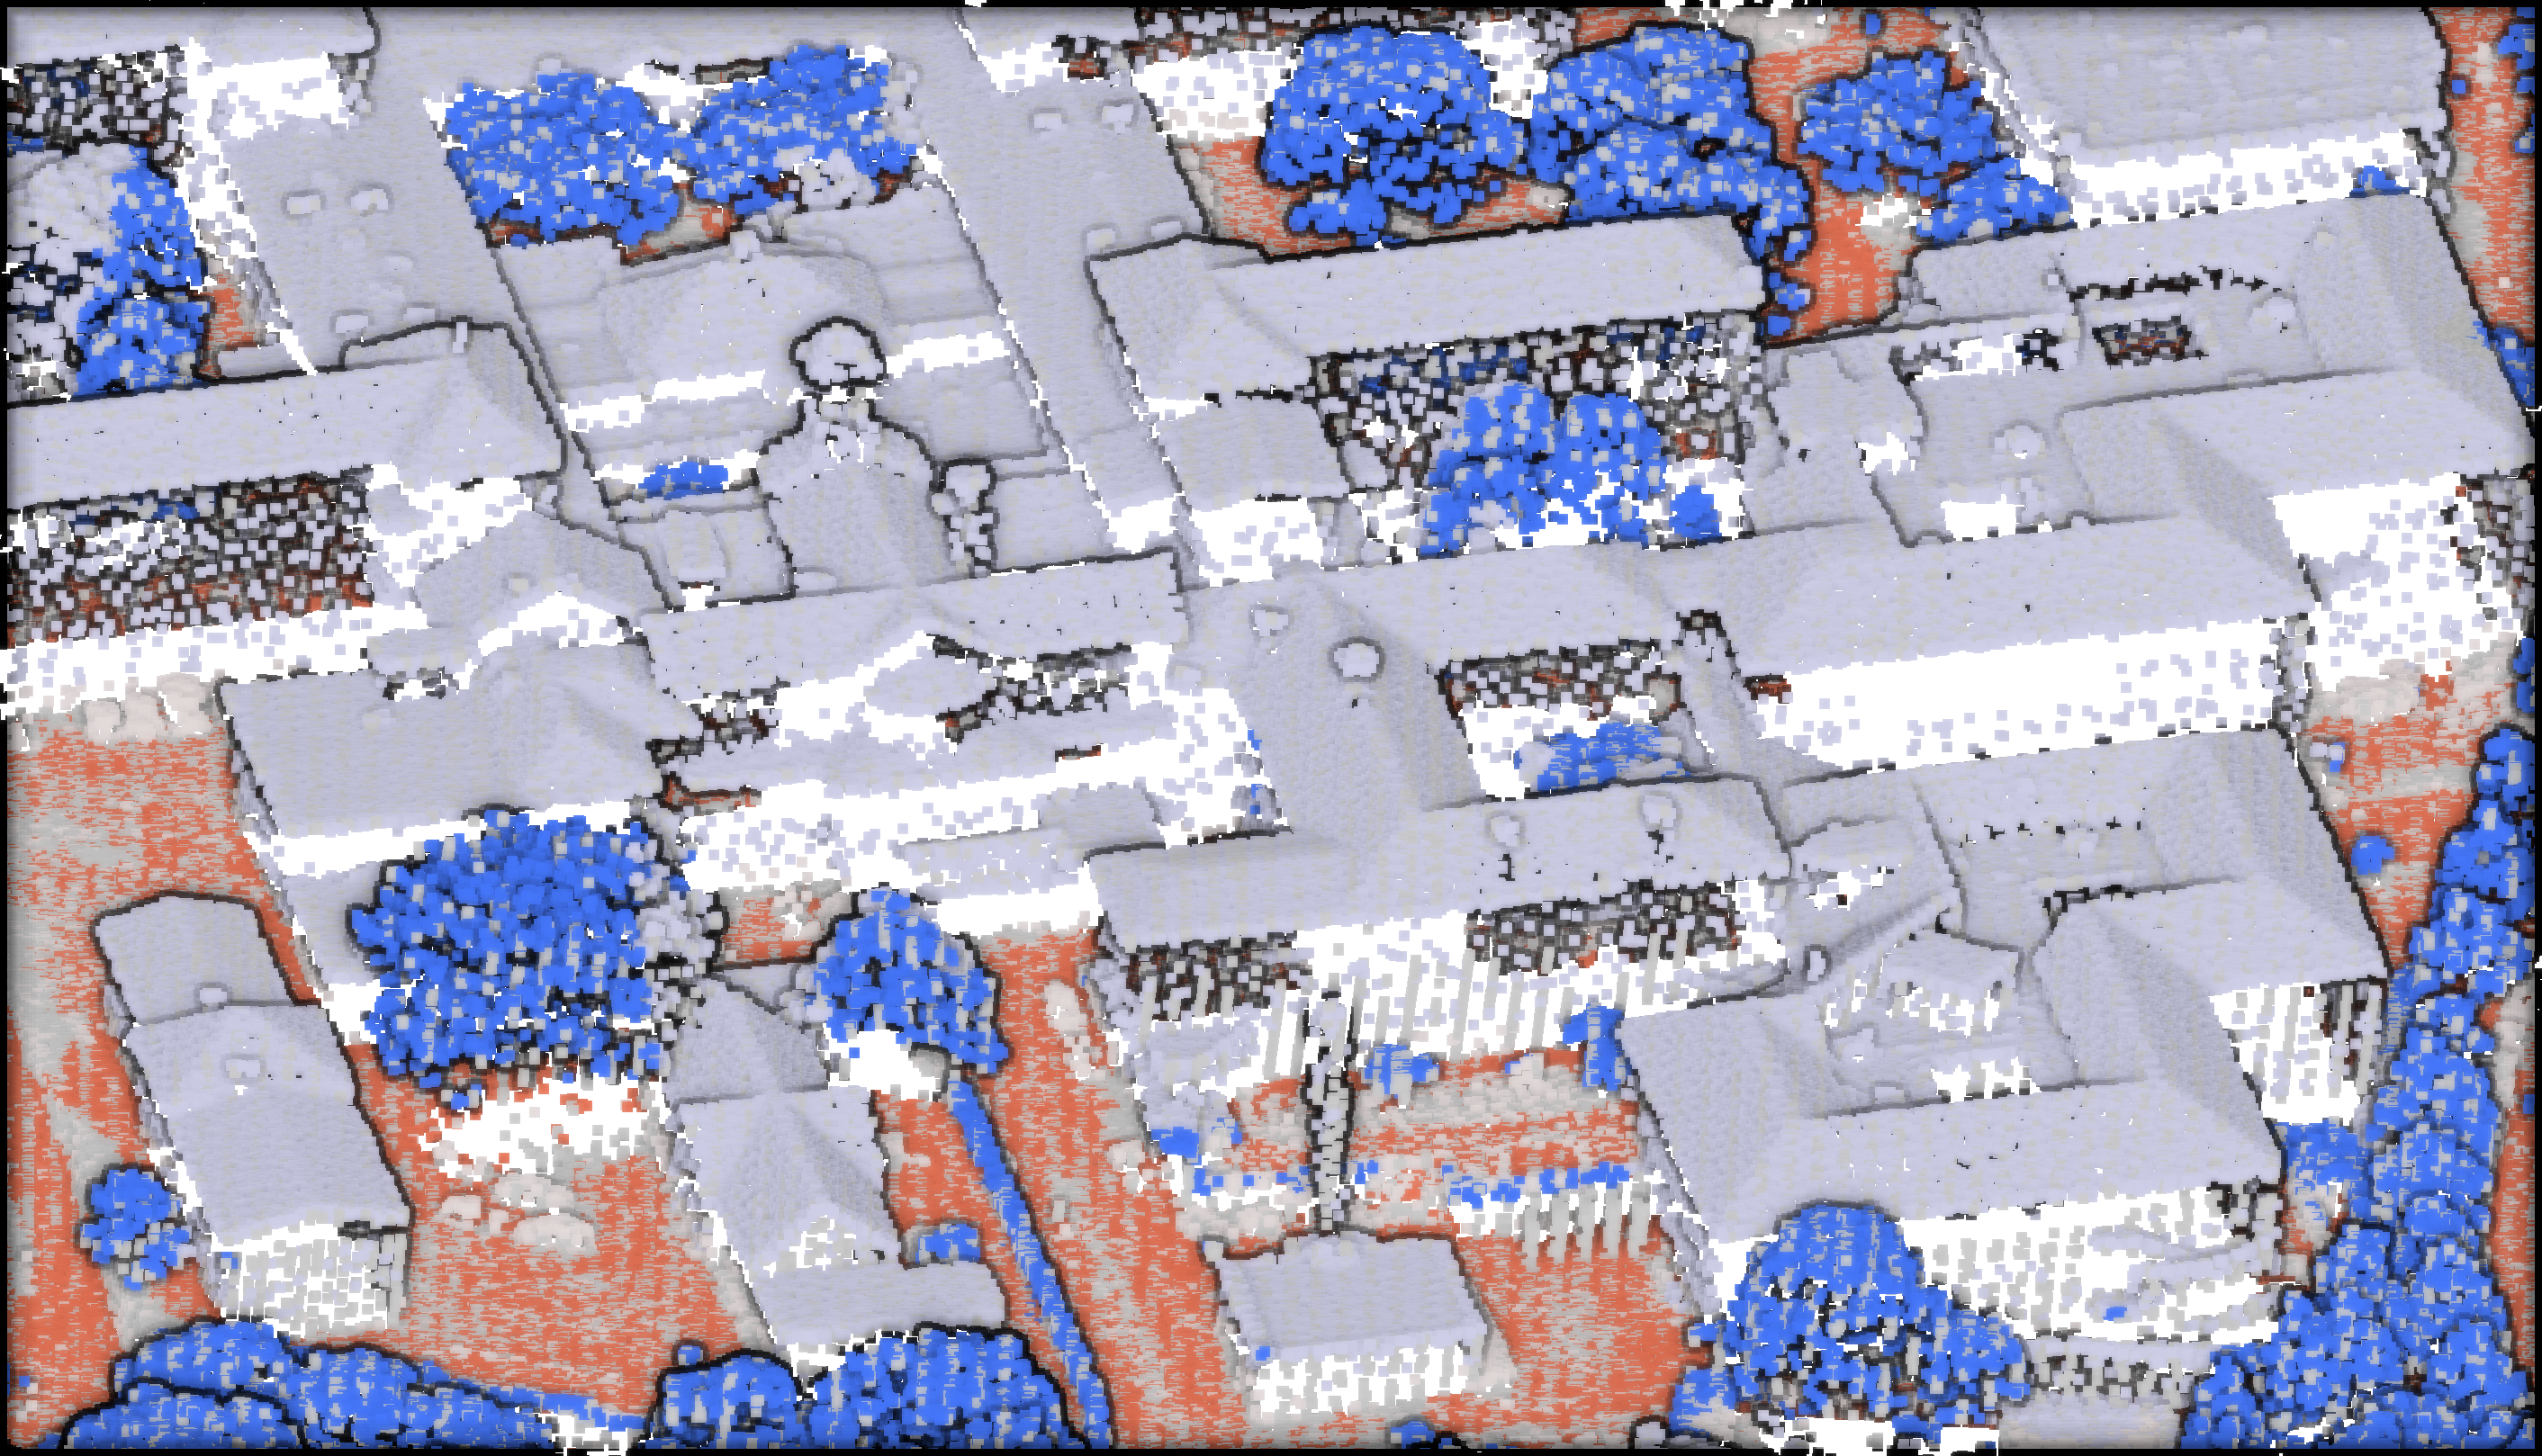
\includegraphics[width=0.8\linewidth]{context/lidar}	
	\end{minipage}%
	\begin{minipage}{0.5\linewidth}
		\centering
		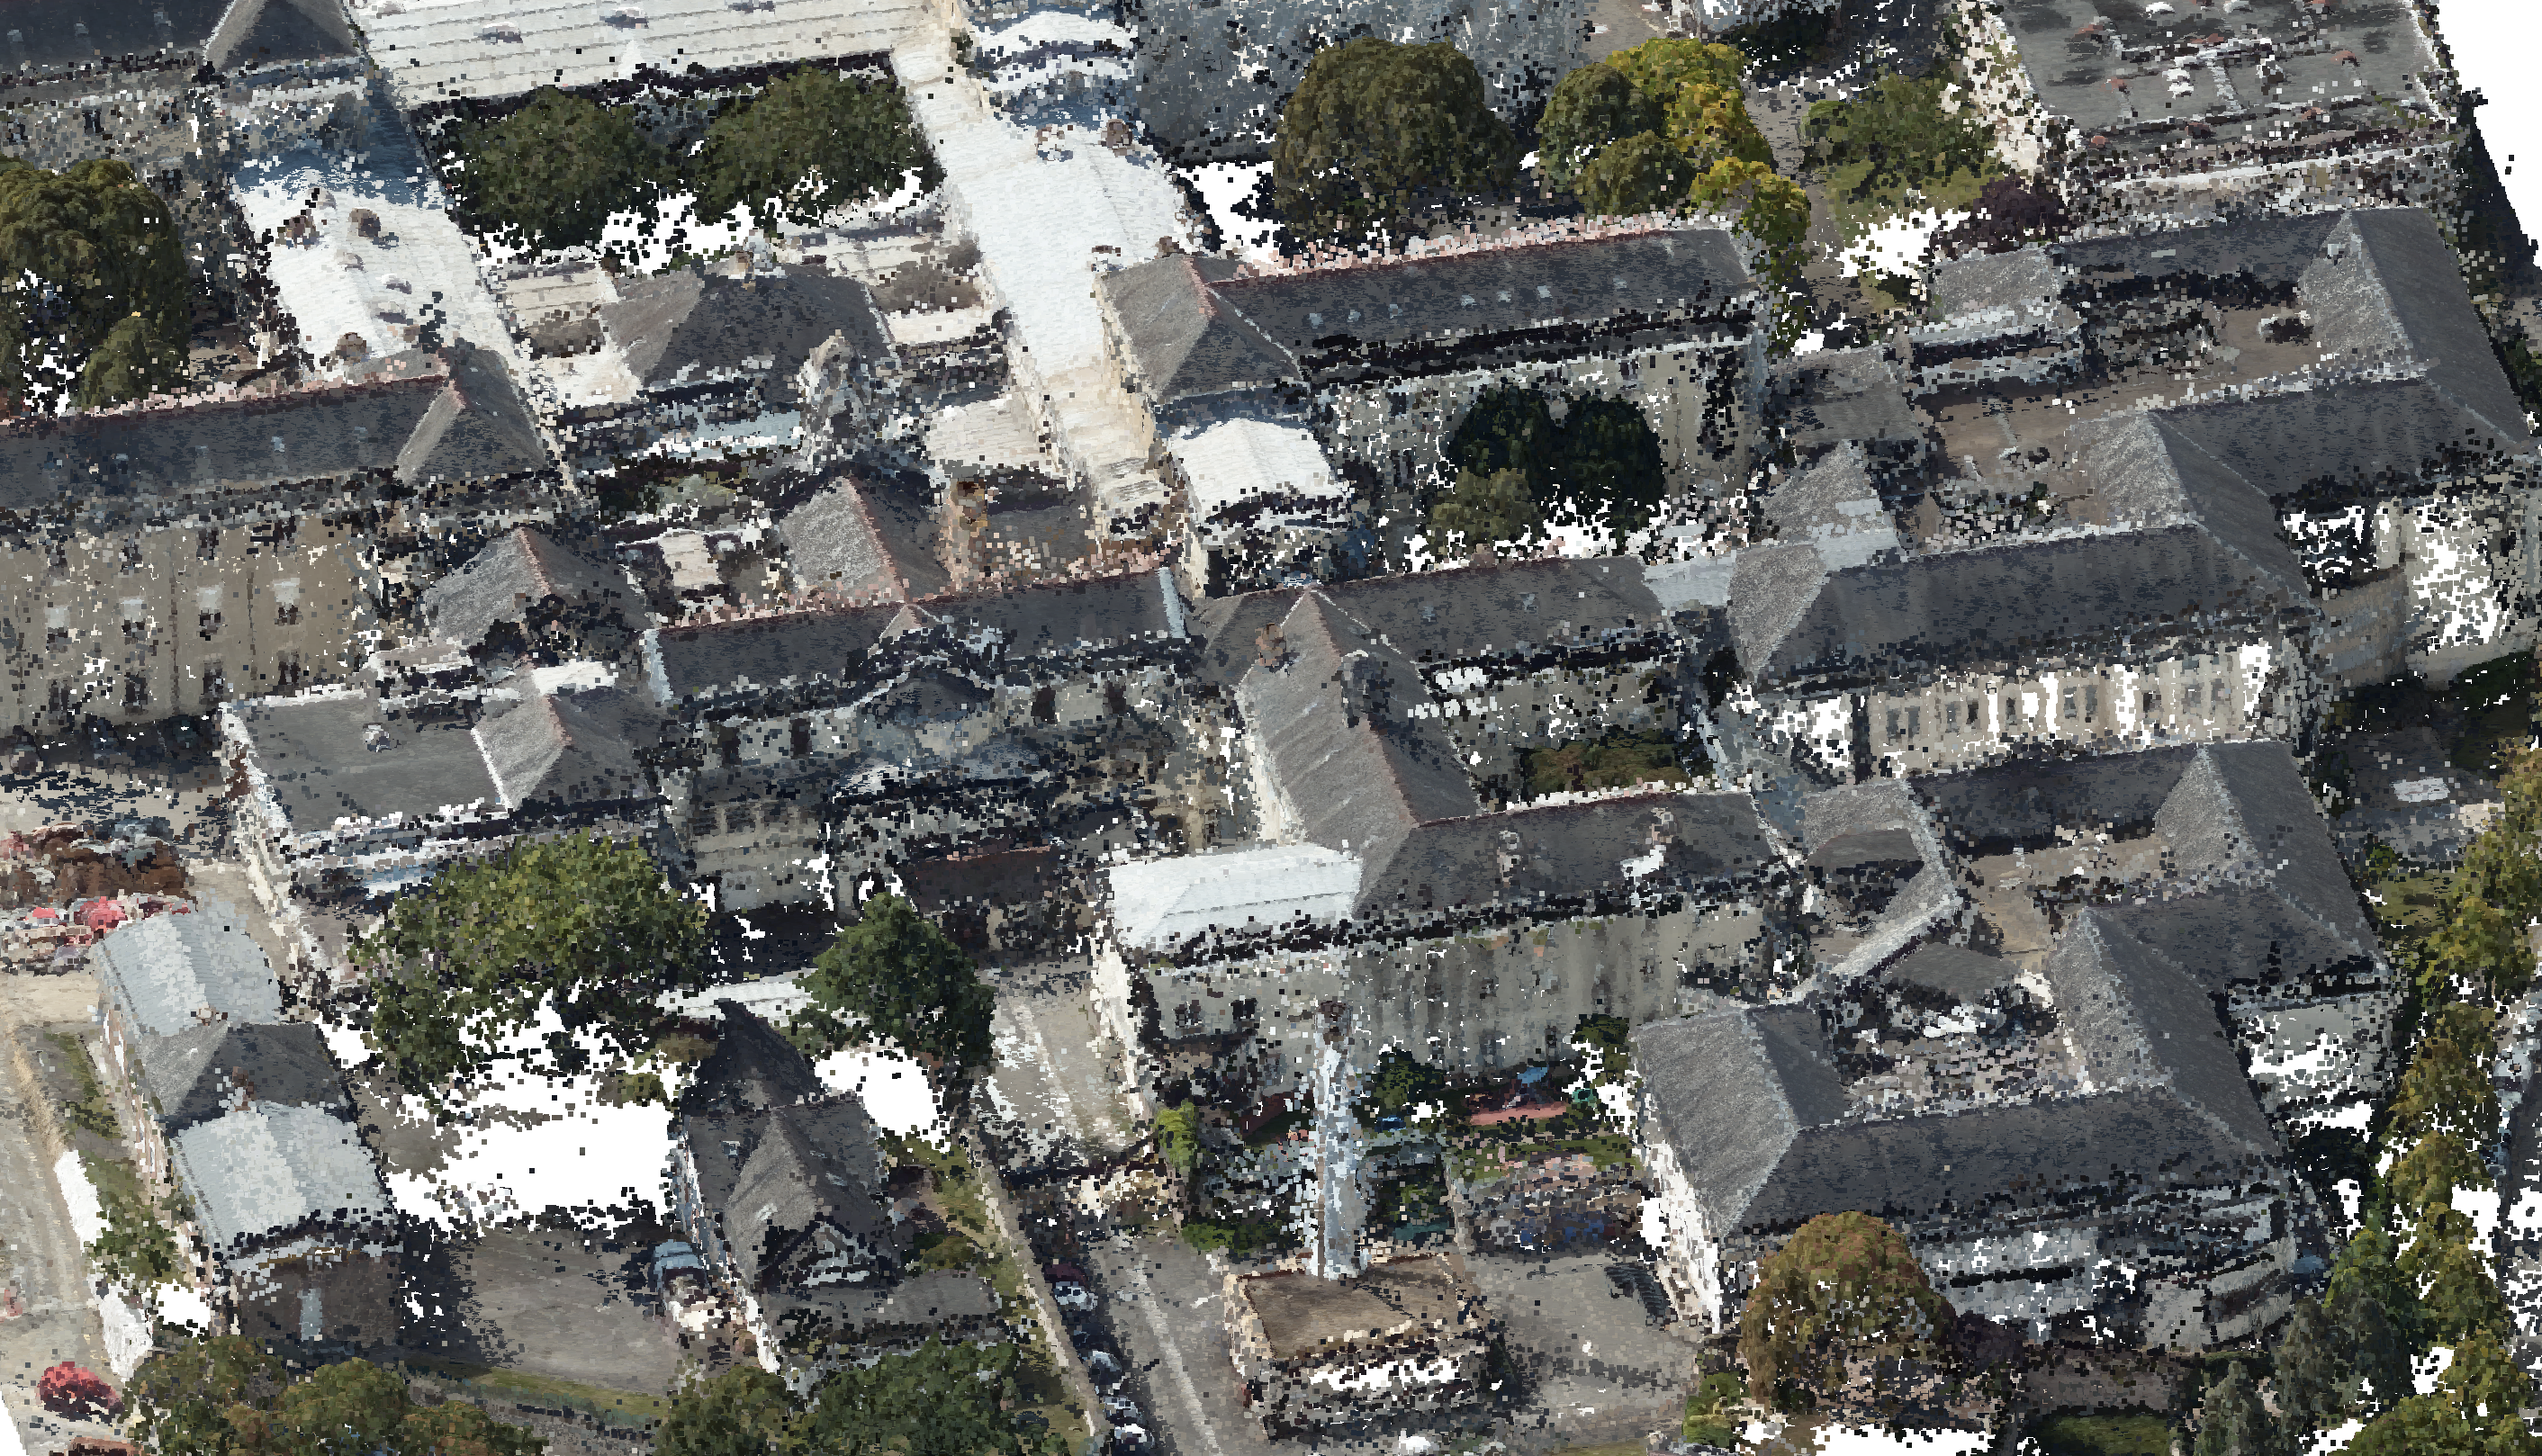
\includegraphics[width=0.8\linewidth]{context/photogrammetry}	
	\end{minipage}%
	
	\blfootnote{Images from \href{https://wingtra.com/drone-photogrammetry-vs-lidar}{Wingtra \ExternalLink}}
\end{frame}

\begin{frame}{Scope of interest}
	\small
	\textbf{Inputs:} Point clouds (LiDAR or Photogrammetry) \\
	\textbf{Semi-automatic} methods of reconstruction \\
	\pause

	\vspace{0.5cm}
	\textbf{Parsimonious representation}
	\begin{itemize}
		\item LOD2 reconstruction
		\item Restricted to buildings
		\item Focus on simplicity \& regularity
	\end{itemize}

	\pause
	\textbf{Dense representation}
	\begin{itemize}
		\item Triangular mesh
		\item Any urban object
		\item Focus on generality \& efficiency
	\end{itemize}
\end{frame}